\documentclass[aspectratio=169]{beamer}
\usetheme{Madrid}
\usecolortheme{default}

\usepackage[utf8]{inputenc}
\usepackage{amsmath,amssymb}
\usepackage{booktabs}
\usepackage{tikz}
\usetikzlibrary{arrows.meta,decorations.pathmorphing,positioning}

\definecolor{deepblue}{RGB}{25,87,140}
\definecolor{warmred}{RGB}{190,70,55}
\setbeamercolor{structure}{fg=deepblue}
\setbeamertemplate{navigation symbols}{}

\title[Shallow-water waves]{Surface waves and the shallow-water limit}
\subtitle{Physics for a hands-on numerical laboratory}
\author{}
\date{}

\newcommand{\unit}[1]{\,\mathrm{#1}}

\begin{document}

\begin{frame}
  \titlepage
\end{frame}

\begin{frame}{What should you be able to do?}
  \begin{itemize}
    \item Read a progressive-wave expression and infer its direction and speed.
    \item Decide whether a surface wave is in the shallow-water regime.
    \item Predict the long-wave speed $c=\sqrt{gH}$ and a travel time.
    \item Explain reflection and the natural period of a closed basin.
    \item Use these ideas to interpret waves driven by an initial disturbance or wind.
  \end{itemize}
  \vfill
  \begin{block}{Laboratory arc}
    Part A: propagation and reflection $\rightarrow$ Part B: varying depth and forcing
    $\rightarrow$ Part C: your own controlled experiment.
  \end{block}
\end{frame}

\begin{frame}{Wave vocabulary}
  \centering
  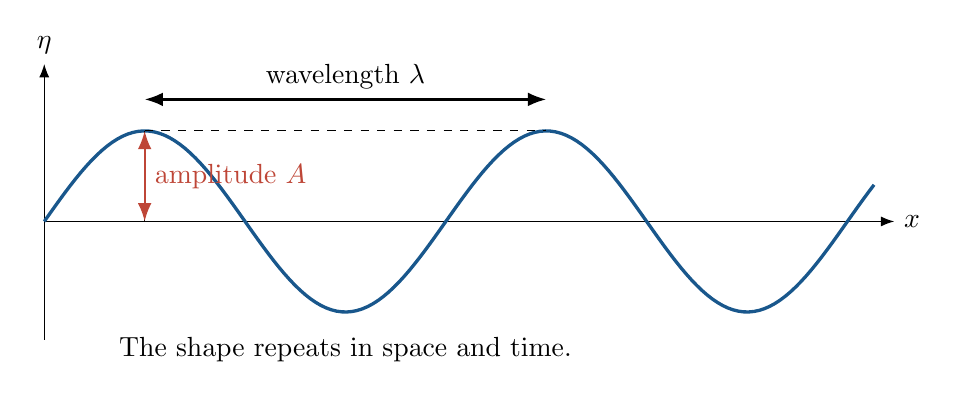
\begin{tikzpicture}[x=0.85cm,y=1.0cm,>=Latex]
    \draw[->] (0,0) -- (12.7,0) node[right] {$x$};
    \draw[->] (0,-1.5) -- (0,2.0) node[above] {$\eta$};
    \draw[deepblue,very thick,domain=0:12.4,samples=160]
      plot (\x,{1.15*sin(60*\x)});
    \draw[dashed] (1.5,0) -- (1.5,1.15);
    \draw[<->,warmred,thick] (1.5,0) -- (1.5,1.15)
      node[midway,right] {amplitude $A$};
    \draw[dashed] (1.5,1.15) -- (7.5,1.15);
    \draw[<->,thick] (1.5,1.55) -- (7.5,1.55)
      node[midway,above] {wavelength $\lambda$};
    \node[below] at (4.5,-1.35) {The shape repeats in space and time.};
  \end{tikzpicture}
  \vfill
  Period $T$; frequency $f_w=1/T$; angular frequency $\omega=2\pi/T$;
  wavenumber $k=2\pi/\lambda$.
\end{frame}

\begin{frame}{A progressive sinusoidal wave}
  \[
    \eta(x,t)=A\cos(kx-\omega t+\phi_0).
  \]
  A fixed phase satisfies
  \[
    kx-\omega t=\hbox{constant}
    \quad\Rightarrow\quad
    \frac{dx}{dt}=\frac{\omega}{k}=c_p.
  \]
  \begin{itemize}
    \item $kx-\omega t$: propagation toward increasing $x$.
    \item $kx+\omega t$: propagation toward decreasing $x$.
    \item $c_p=\omega/k=\lambda/T$ is the phase speed.
  \end{itemize}
  A crest is a particular phase, not a marked parcel of water.
\end{frame}

\begin{frame}{Exercise 1: read the wave}
  Consider, with $x$ in metres and $t$ in seconds,
  \[
    \eta(x,t)=0.15\cos\left(\frac{2\pi x}{200}-\frac{2\pi t}{20}\right)\unit{m}.
  \]
  Find:
  \begin{enumerate}
    \item amplitude, wavelength, and period;
    \item propagation direction and phase speed;
    \item $\eta$ at $x=50\unit{m}$ and $t=2\unit{s}$.
  \end{enumerate}
  \vfill
  Work with a neighbour for 4 minutes. Keep units in every answer.
\end{frame}

\begin{frame}{Exercise 1: solution}
  \begin{align*}
    A &= 0.15\unit{m}, & \lambda &= 200\unit{m}, & T &= 20\unit{s},\\
    c_p &= \frac{\lambda}{T}=10\unit{m\,s^{-1}}.&&&
  \end{align*}
  The minus sign gives propagation toward increasing $x$.
  At $x=50\unit{m}$ and $t=2\unit{s}$,
  \[
    kx-\omega t=\frac{\pi}{2}-\frac{\pi}{5}=\frac{3\pi}{10},
    \qquad
    \eta\approx0.088\unit{m}.
  \]
  \begin{alertblock}{Check}
    A surface displacement cannot exceed the stated amplitude $0.15\unit{m}$.
  \end{alertblock}
\end{frame}

\begin{frame}{What moves with a wave?}
  \begin{columns}[T]
    \column{0.53\textwidth}
      \begin{itemize}
        \item Phase and energy can travel across the basin.
        \item Individual parcels usually oscillate around a mean position.
        \item A long wave has both surface displacement and horizontal current.
        \item Net transport can occur, but it is not identical to the phase motion.
      \end{itemize}
    \column{0.43\textwidth}
      \centering
      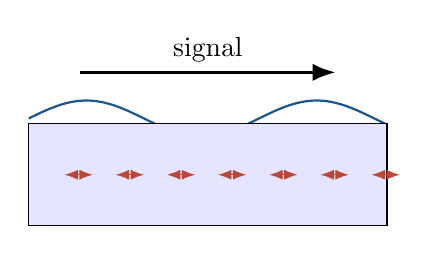
\begin{tikzpicture}[x=0.65cm,y=0.65cm,>=Latex]
        \draw[deepblue,thick,domain=0:7,samples=100]
          plot (\x,{0.35*sin(80*\x)+2.1});
        \draw[fill=blue!10] (0,0) rectangle (7,2);
        \foreach \x in {0.7,1.7,...,6.7}{
          \draw[<->,warmred] (\x,1) -- +(0.55,0);
        }
        \draw[->,very thick] (1,3) -- (6,3) node[midway,above] {signal};
      \end{tikzpicture}
  \end{columns}
\end{frame}

\begin{frame}{Surface gravity is the restoring force}
  A displaced free surface creates a horizontal pressure gradient.
  Gravity accelerates water away from high surface elevation.
  \[
    \frac{\partial u}{\partial t}=-g\frac{\partial\eta}{\partial x}
    \quad\hbox{(simplest linear, non-rotating form).}
  \]
  \begin{block}{Two geometric scales matter}
    Water depth $H$ and wavelength $\lambda$ determine whether the bottom affects
    the entire water-column motion.
  \end{block}
\end{frame}

\begin{frame}{The surface-gravity-wave dispersion relation}
  For linear waves over uniform depth,
  \[
    \boxed{\omega^2=gk\tanh(kH)}.
  \]
  \begin{itemize}
    \item It connects frequency, wavelength, gravity, and water depth.
    \item The dimensionless parameter $kH=2\pi H/\lambda$ identifies the regime.
    \item If $\omega/k$ depends on $k$, different wavelengths propagate at
      different phase speeds: the waves are dispersive.
  \end{itemize}
\end{frame}

\begin{frame}{Deep and shallow limits}
  \begin{columns}[T]
    \column{0.48\textwidth}
      \begin{block}{Deep water: $kH\gg1$}
        $\tanh(kH)\approx1$
        \[
          \omega^2\approx gk,
          \qquad c_p\approx\sqrt{\frac{g}{k}}.
        \]
        Speed depends on wavelength.
      \end{block}
    \column{0.48\textwidth}
      \begin{block}{Shallow water: $kH\ll1$}
        $\tanh(kH)\approx kH$
        \[
          \omega^2\approx gHk^2,
          \qquad c_p\approx\sqrt{gH}.
        \]
        Speed is independent of wavelength.
      \end{block}
  \end{columns}
  \vfill
  ``Shallow'' compares depth with wavelength, not with a swimmer or ship.
\end{frame}

\begin{frame}{Exercise 2: classify the waves}
  Estimate $kH=2\pi H/\lambda$ and classify each case.
  \begin{center}
  \begin{tabular}{lrr}
    \toprule
    Example & $H$ & $\lambda$ \\
    \midrule
    Long ocean disturbance & $4000\unit{m}$ & $200\unit{km}$ \\
    Wind wave on a shelf & $50\unit{m}$ & $100\unit{m}$ \\
    Basin-scale tide & $100\unit{m}$ & $1000\unit{km}$ \\
    \bottomrule
  \end{tabular}
  \end{center}
  Which examples can a non-dispersive shallow-water model represent most directly?
\end{frame}

\begin{frame}{Exercise 2: solution}
  \begin{center}
  \begin{tabular}{lrl}
    \toprule
    Example & $kH$ & Interpretation \\
    \midrule
    Long ocean disturbance & $0.126$ & shallow-water approximation \\
    Wind wave on a shelf & $3.14$ & not shallow; dispersive \\
    Basin-scale tide & $0.00063$ & strongly shallow \\
    \bottomrule
  \end{tabular}
  \end{center}
  \begin{block}{Important}
    A tsunami and a tide can both satisfy shallow-water dynamics even though one
    begins as an initial disturbance and the other is continuously forced.
  \end{block}
\end{frame}

\begin{frame}{Break and reset}
  \centering
  \Large 10-minute break
  \vfill
  \normalsize After the break: speed, reflection, bathymetry, and forcing.
\end{frame}

\begin{frame}{Where does $c=\sqrt{gH}$ come from?}
  In one horizontal dimension, the linear non-rotating shallow-water equations are
  \[
    \frac{\partial u}{\partial t}=-g\frac{\partial\eta}{\partial x},
    \qquad
    \frac{\partial\eta}{\partial t}=-H\frac{\partial u}{\partial x}.
  \]
  Differentiate and combine:
  \[
    \frac{\partial^2\eta}{\partial t^2}
    =gH\frac{\partial^2\eta}{\partial x^2}.
  \]
  This is a wave equation with speed
  \[
    \boxed{c=\sqrt{gH}}.
  \]
\end{frame}

\begin{frame}{Exercise 3: depth and travel time}
  Compare a long wave over depths $H_1=100\unit{m}$ and $H_2=400\unit{m}$.
  \begin{enumerate}
    \item Calculate both speeds.
    \item Find the speed ratio $c_2/c_1$ before using a calculator.
    \item Estimate the travel time across $1000\unit{km}$ in each case.
  \end{enumerate}
  Use $g=9.81\unit{m\,s^{-2}}$.
\end{frame}

\begin{frame}{Exercise 3: solution}
  \begin{align*}
    c_1 &= \sqrt{9.81\times100}=31.3\unit{m\,s^{-1}},\\
    c_2 &= \sqrt{9.81\times400}=62.6\unit{m\,s^{-1}},\\
    \frac{c_2}{c_1} &= \sqrt{\frac{400}{100}}=2.
  \end{align*}
  For $L=1000\unit{km}$, $t=L/c$ gives approximately
  \[
    t_1=8.9\unit{h},\qquad t_2=4.4\unit{h}.
  \]
  Deeper water gives faster long waves.
\end{frame}

\begin{frame}{Reflection from a vertical coast}
  \begin{columns}
    \column{0.55\textwidth}
      At a solid wall, normal velocity must vanish:
      \[
        u_n=0.
      \]
      An incident and reflected wave combine to satisfy this condition.
      \begin{itemize}
        \item Normal velocity reverses sign.
        \item Surface displacement reflects without a sign reversal at a rigid wall.
        \item Incident and reflected waves may form a standing pattern.
      \end{itemize}
    \column{0.40\textwidth}
      \centering
      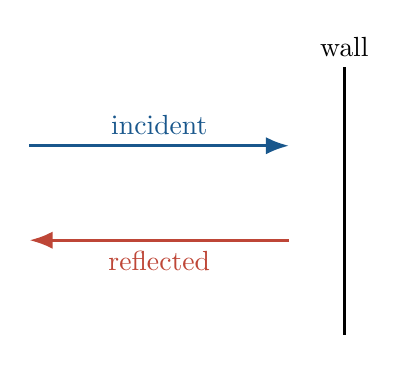
\begin{tikzpicture}[>=Latex]
        \draw[very thick] (4,-1.2) -- (4,2.2) node[above] {wall};
        \draw[->,deepblue,very thick] (0,1.2) -- (3.3,1.2)
          node[midway,above] {incident};
        \draw[->,warmred,very thick] (3.3,0) -- (0,0)
          node[midway,below] {reflected};
      \end{tikzpicture}
  \end{columns}
\end{frame}

\begin{frame}{Standing waves and basin seiches}
  Two equal waves moving in opposite directions give
  \begin{align*}
    \eta &= A\cos(kx-\omega t)+A\cos(kx+\omega t)\\
         &=2A\cos(kx)\cos(\omega t).
  \end{align*}
  The spatial pattern has fixed nodes and antinodes.
  For the fundamental mode of a closed rectangular basin,
  \[
    \lambda_1=2L,
    \qquad
    T_1=\frac{2L}{\sqrt{gH}}.
  \]
  Repeated forcing near a natural period can produce a large response.
\end{frame}

\begin{frame}{Exercise 4: a basin timescale}
  A closed basin has length $L=600\unit{km}$ and uniform depth $H=100\unit{m}$.
  \begin{enumerate}
    \item Estimate its fundamental seiche period.
    \item If the basin length doubles at the same depth, what happens to the period?
    \item If depth quadruples at the same length, what happens to the period?
  \end{enumerate}
\end{frame}

\begin{frame}{Exercise 4: solution}
  \[
    c=31.3\unit{m\,s^{-1}},
    \qquad
    T_1=\frac{2(600\times10^3)}{31.3}
       \approx10.6\unit{h}.
  \]
  \begin{itemize}
    \item Doubling $L$ doubles $T_1$.
    \item Quadrupling $H$ doubles $c$ and therefore halves $T_1$.
  \end{itemize}
  These are hypotheses that can be tested directly in Part A or Part C.
\end{frame}

\begin{frame}{What varying depth changes}
  If $H=H(x,y)$, the local long-wave speed is
  \[
    c(x,y)=\sqrt{gH(x,y)}.
  \]
  \begin{itemize}
    \item A wave slows as it enters shallower water.
    \item At approximately conserved frequency, its wavelength shortens.
    \item Amplitude can change through shoaling, convergence/divergence, and reflection.
    \item An abrupt depth change usually reflects more strongly than a gentle change.
  \end{itemize}
  Part B isolates these effects with a broad pulse and virtual gauges.
\end{frame}

\begin{frame}{Initial disturbances and continuous forcing}
  \begin{columns}[T]
    \column{0.48\textwidth}
      \begin{block}{Initial-value problem}
        Specify $\eta,u,v$ at $t=0$, then remove external forcing.
        \begin{itemize}
          \item uplift-like pulse
          \item released basin displacement
          \item initial current
        \end{itemize}
      \end{block}
    \column{0.48\textwidth}
      \begin{block}{Forced problem}
        Apply stress, pressure, or mass input through time.
        \begin{itemize}
          \item wind setup and release
          \item periodic tidal potential
          \item moving storm-like forcing
        \end{itemize}
      \end{block}
  \end{columns}
  The same shallow-water dynamics can connect these different applications.
\end{frame}

\begin{frame}{What the numerical model represents}
  \begin{columns}[T]
    \column{0.49\textwidth}
      \begin{block}{Included}
        \begin{itemize}
          \item depth-averaged $u,v$ and free surface $\eta$
          \item rectangular, fully wet domain
          \item uniform or variable positive depth
          \item solid side walls
          \item wind, pressure, mass, and periodic forcing
          \item optional rotation and damping
        \end{itemize}
      \end{block}
    \column{0.49\textwidth}
      \begin{alertblock}{Not included}
        \begin{itemize}
          \item vertical structure
          \item dry land and moving shoreline
          \item wave breaking and run-up
          \item coastal inundation or damage
          \item short-wave dispersion
          \item resolved bottom boundary layer
        \end{itemize}
      \end{alertblock}
  \end{columns}
\end{frame}

\begin{frame}[fragile]{Course installation}
  After the course release is published:
  \begin{verbatim}
python -m pip install "shallowwater==0.1.4"
  \end{verbatim}
  Optional numba acceleration:
  \begin{verbatim}
python -m pip install "shallowwater[numba]==0.1.4"
  \end{verbatim}
  Check the environment in a notebook:
  \begin{verbatim}
import shallowwater
print(shallowwater.backend_info())
  \end{verbatim}
  Numba is optional; its first run may pause for compilation.
\end{frame}

\begin{frame}{Your opening Part A prediction}
  \centering
  \Large
  A broad elevation is placed in a uniform-depth, closed rectangular basin.

  \vspace{1cm}
  What happens after release?

  \vspace{0.6cm}
  \normalsize
  Predict the propagation direction, speed scale, and what occurs at the wall
  before running the notebook.
\end{frame}

\end{document}
